\newcommand{\todo}[1]{{\bf [TODO #1]}}

{\bf A INCLURE DANS ``WP 3.4 - Developing a new annotation platform''}\\


As reported in QPR10, LIPN continues to develop a new annotation platform based on UIMA. During the last period, LIPN has
\begin{enumerate}
\item studied some conceptual issues about concurrent annotations,
\item alsmost achieved the first version of the platform,
\item started to establish some guidelines to use current components and develop future ones.
\end{enumerate}
\medskip

{\bf Design issues}
\medskip

Firstly the LIPN generic Type System (TS) has been slightly modified in the last period: {\tt Relation} types now refer to {\tt GenericAnnotation} types instead of {\tt Segment} (see QPR10). There was actually no reason to restrict the range of annotations that a {\tt Relation} can refer to; in particular a relation annotation can concern other relation annotations (for example a tree structure should be represented with such {\tt Relation} types).

\begin{figure}[htbp]
\begin{center}
\scalebox{.7}[.6]{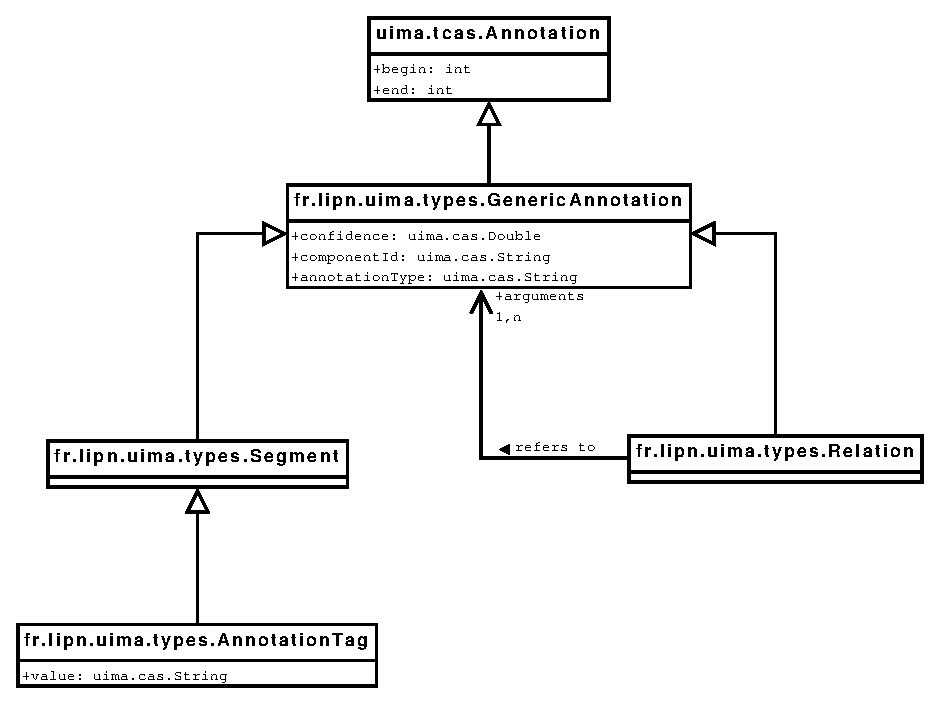
\includegraphics{TS05.eps}}
\end{center}
\caption{The updated LIPN Type System \label{fig-LIPN-TS}}
\end{figure}


LIPN has carried out some conceptual work to make the platform fit the needs defined in QPR10: LIPN wants to build a generic and modular platform, which is also able to handle concurrent annotations (see QPR10). This sometimes requires to find technical solutions for some issues. In particular, the ability to handle concurrent annotations can not be straightforwardly implemented. it requires to define a mechanism to deal with this feature at different levels.

%\begin{itemize}
%\item 
At the lower level (probably in a package or class which embeds all technical details about concurrent annotation access, providing methods to be called by the annotators), the question is: how two concurrent series of annotations are represented in the CAS\footnote{Common Analysis Structure: it is the main UIMA data structure containing the document data, the Type System and the annotations.}? If possible, this representation should be efficient, and convenient access to this level should be provided.

At the annotator level, there are cases where the annotator is aware that it is working with concurrent annotations, but sometimes one simply wants to run a standard annotator on one serie of annotations among several concurrent ones. Is it possible to access concurrent annotations ``transparently'', i.e. in the same way that usual UIMA annotations? How and in which cases does an annotator access to the ``concurrent side'' of annotations?

At the higher/user\footnote{It is worth noticing that in the UIMA framework it is sometimes hard to precisely define the {\em user} level, because this user may be either someone who only runs the component on some document, or someone who develops a new component which uses its output, or someone who includes this component in a pipe process: these different ``users'' do not have exactly the same viewpoint and knowledge about the component, and the developer must take all these into account.} level, it is necessary to provide a way to control the series of concurrent annotations: if the CAS contains different series of annotations,  it must be possible to tell a ``simple'' annotator (which reads a single set of annotations and write some new ones) which serie it should read, and possibly if the annotations it writes should be considered as a concurrent serie.

%\end{itemize}

These questions are still studied, but several general ideas are proposed:
%\item About representing concurrent annotations, several possibilities are considered:
\begin{itemize}
\item The first idea consists in using a feature like {\tt componentId} (see figure \ref{fig-LIPN-TS}) to distinguish between different series of annotations. This is simple and sufficiant for most cases, as soon as such a feature can be parameterized by the user (since it should be possible to write different series of annotations with the same component). Nevertheless this solution can not handle complex cases, like concurrent annotations related to syntactic ambiguities created in the same component, for example.
\item Another idea consists in using UIMA possible features types that a type can contain. In particular it is possible to define a list of annotation as type for a feature, which means simply that an annotation can contain some other annotations. In this approach a special type of annotation indicating ``concurrency'' would be set, covering exactly the section of the document it is related to; each such annotation would contain the serie of annotations. Among the possible drawbacks, it is harder to link an annotation included in such a list to any other element (text or annotation) outside the list.
\item Using UIMA's concept of {\em view}: originally designed to represent the same document in different ways (e.g. with/without HTML tags, or the same content in different languages), views seem to be a good approach: here also, for every concurrent annotation concerning the document (contained in the main view), a special annotation indicating ``concurrency'' would be set; it would cover exactly the section of the document it is related to, and would contain an identifier for the view in which the remaining information is stored. This way views would be used as a generic pointers mechanism, and that would permit to represent any kind of complex annotations, since it is possible to nest such pointers as much as needed. As a possible drawback, given an annotation it would probably be harder to get back to the original text it describes (and to its indexes in this text).
\end{itemize}



{\bf Implementation}
\medskip



The core components are now almost achieved. They consist in:
\begin{enumerate}
\item A module devoted to interface with external programs, essentially to deal with 
\begin{itemize}
\item The environment in which the program is called, including controlling the process, handling errors, charset encoding, input and output transmission.
\item Input and output format issues (representation, conversions).
\end{itemize}
This module was described in QPR10, it has been more deeply tested and enhanced.
\item Some packages providing implementation for the common tasks of LIPN UIMA annotators. these are not only provided for convenience, but also to ensure that all annotators follow some general guidelines, in order to strengthen consistency and compatibility among components.
\item The annotators components themselves: TreeTagger (part-of-speech tagger) and the YaTeA terminology extractor were added during the last period, as planed in QPR10.
\end{enumerate}

A certain amount of time has been spent to deal with concurrency (now in the usual sense, i.e. when different threads run at the same time): as presented in QPR10, LIPN builds components which are wrappers for existing tools. These external programs are called during the process: the UIMA annotator task thus consists in extracting data from the CAS, formatting it, sending it to the program as input, and then to receive the program output, reading it and adding new annotations to the CAS. For the sake of efficiency the data is transmitted ``on the fly'' whenever possible: indeed, a lot of tools read their input as a stream ({\em stdin}) and write their output as another one ({\em stdout}). Transmitting data on the fly avoids storing it as a file or in memory: firstly this saves space, and (memory) space may sometimes be a problem with very large documents. Secondly this is a gain of time, since both in input and output the receiver does not have to wait for the sender to transmit the whole data (the gain is even more important compared to storing the data as a file, since disk access are very time consuming).

Threading data transmission when calling an external program requires quite careful programming and testing, but it is not very hard. But using concurrency when accessing the CAS is on the contrary quite challenging: actually UIMA is designed (and even quite powerful) to deal with different threads running several (instances of) annotators in the same time, but it is not intended to handle concurrency {\em inside} a single annotator. Thus all CAS accesses have to be protected (synchronized), which is in fact quite tedious. LIPN had then to develop an approach and tools to embed most thread-related code, in order to make things easier for the annotator developer. These tools are now achieved, and have been thoroughly tested (since concurrency bugs are a real pain to track).

Finally LIPN now prepares a first complete version of this platform. In order to package it in a convenient way, Maven\footnote{\url{http://maven.apache.org}} has been used. Since this platform is quite complex, due both to UIMA mechanisms and to LIPN's own approach, a complete documentation is planed, and some examples will also be included. Some questions arise during this final step: for example, there are choices to make between ease of use and the policy decided about the Type System. There is also often a trade-off between the UIMA ``component sharing philosophy'' and the actual local needs of the LIPN team, or between the genericity of the annotators (allowing maximal parameterization) and the ``pipe viewpoint'' (requiring more simple components). Fortunately UIMA provides various ways to ``see'' a component, in particular using the different possible levels to call it: a component can be called and parameterized programmatically, or using a totally customizable descriptor, or the developer can provide a default descriptor hiding most details of parameters.


\bigskip





{\bf A INCLURE DANS ``OBJECTIVES FOR THE NEXT PERIOD''}

For the next period LIPN will
\begin{itemize}
\item Continue to test the platform in various cases, possibly correct/improve code.
\item Achieving documentation, including:
\begin{itemize}
\item a user guide, which will explain LIPN generic approach and help the user understand how to process documents in this framework, in particular by providing examples.
\item a developer guide which detail implementation choices and provide guidelines for further development of annotators in LIPN.
\end{itemize}
Documentation is a quite complex task because there are lot of ways to develop and use components in the UIMA framework. Of course this is an advantage, but it may be a bit confusing on the user side, and on the developer side it is important to maintain consistency among the different LIPN components.
\item Package the modules in a reliable and convenient way.
\item \todo{À VERIFIER} Depending on time and priorities, maybe develop new / integrate existing annotators. There are different ideas that LIPN may study:
\begin{itemize}
\item A term tagger, because it is a very useful component for LIPN,
\item A syntaxic parser, which would be useful of course but would also have another interest: it is indeed interesting to create/test concurrent annotations in a context where there are possibly different nested structures (due to syntactic ambiguities),
\item A customizable tokenizer, based on applying some rules defined by the user.
\end{itemize}
\end{itemize}

